\section{Resultados}

Aclaraciones:	\\
\indent	Para la obtención de los resultados hicimos traceroutes a direcciones ips pertenecientes a sitios web hosteados en Europa. También experimentamos bastante con sitios de Asia, Oceania y Africa, aunque estos no fueron utilizados para los resultados ya que no obtuvimos enlaces transatlánticos distintos a los obtenidos con los sitios Europeos y notamos un mayor tiempo de respuesta hacia estos.	\\
\indent	Una vez obtenidos los enlaces, para obtener la variación del RTT hacia los mismos a lo largo del día realizamos 20 pings sucesivos a cada enlace, cada 1 hora, durante 24 horas, y consideramos el promedio de esos pings. En caso de obtener un timeout entre los 20 pings, dicho ping fue descartado a la hora de sacar el promedio.

\subsection{Enlaces transatlánticos}

%~ http://maps.googleapis.com/maps/api/staticmap?zoom=1&size=600x400&scale=2&sensor=false&maptype=roadmap
%~ 	&markers=label:1|37.9283,-122.0566
%~ 	&markers=label:2|-35.28,149.22
%~ 	&path=color:0xff0000|weight:2|37.9283,-122.0566|-35.28,149.22

%~ http://maps.googleapis.com/maps/api/staticmap?zoom=1&size=600x400&scale=2&sensor=false&maptype=roadmap
%~ 	&markers=label:1|25.77427,-80.19366
%~ 	&markers=label:2|51.50853,-0.12574
%~ 	&markers=label:3|40.71427,-74.00597
%~ 	&path=color:0xff0000|weight:2|25.77427,-80.19366|51.50853,-0.12574
%~ 	&path=color:0xff0000|weight:2|40.71427,-74.00597|51.50853,-0.12574

\begin{figure}[H]
\begin{center}
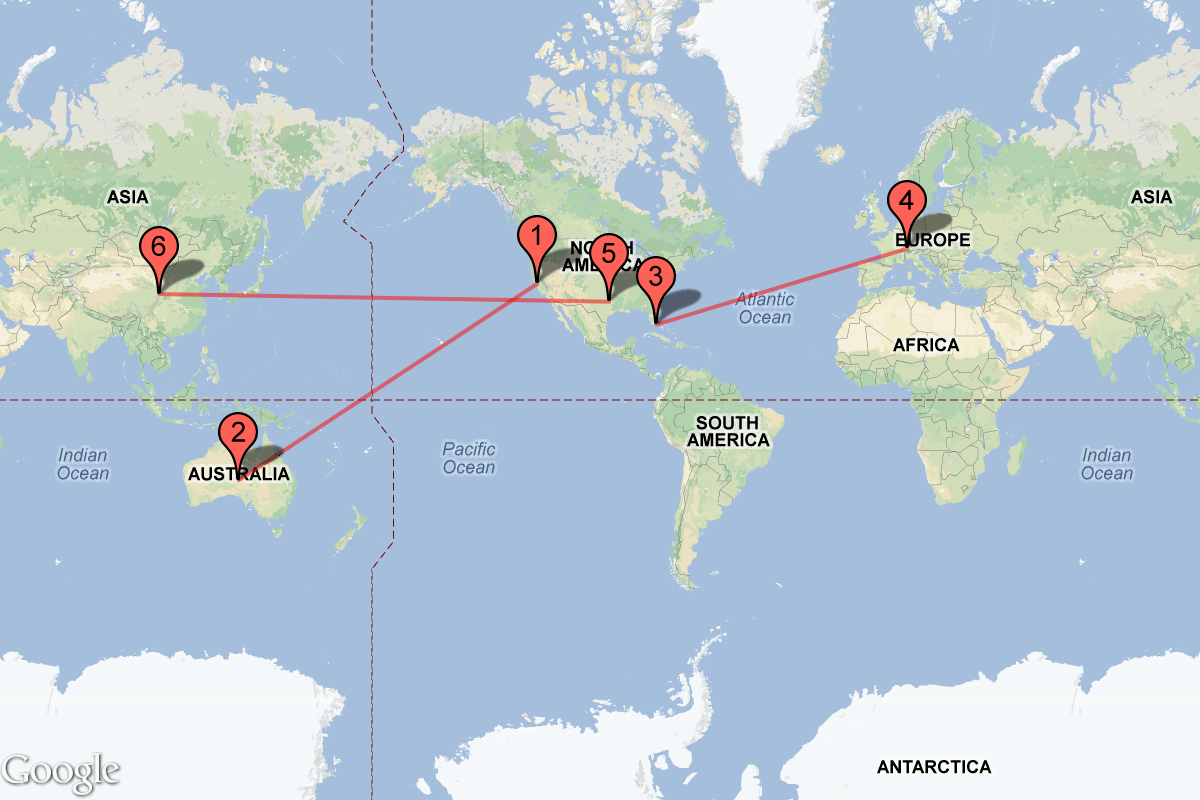
\includegraphics[width=17cm]{enlaces.png}
\end{center}
\caption{Enlaces transatlánticos} \label{figura1}
\end{figure}

A pesar de realizar muchas pruebas con traceroute a varias universidades al otro lado del Atl'antico, s'olo pudimos observar 2 enlaces transatl'anticos diferentes, uno al apuntar a la University of London, que utiliz'o un enlace entre Miami y Londres, y el otro al apuntar a la Universidade de Cabo Verde, que usa un enlace entre Nueva York y Londres. El resto de los sitios probados usaba uno esos dos enlaces, o los datos que obteniamos no eran coherentes con lo esperado por un enlace submarino.

\noindent \begin{center} \begin{tabular}{| c | c | c | c | c |} \hline 
Pin 	& 	 Dirección IP 	 & 	 Coordenadas 		 & 	 Distancia total recorrida hasta él en Km 	 & 	 RTT mínimo en ms 	\\ \hline 
1 	 	& 	213.200.84.37  & (25.77427,-80.19366)	 & 	 			7097			 & 	 	 	35.485			\\ \hline 
2 		& 	141.136.107.41 & (51.50853,-0.12574)	 & 	 			11130			 & 	 		55.65			\\ \hline 
3 	 	& 	94.142.122.217 & (40.71427,-74.00597)	 & 	  		8527			 & 	 		42.635			\\ \hline 
4 	 	& 	84.16.12.21		 & (51.50853,-0.12574)	 & 	  		11130			 & 	  	55.65				\\ \hline 
5 	 	& 	  				 & 	  					 & 	  											 & 	  					\\ \hline 
6 	 	& 	  				 & 	 				 	 & 	  											 & 	  					\\ \hline 
%~ 3 	 & 	 195.22.199.109 	 & 	 (25.7743,-80.1937) 	 & 	 7887.31191972 	 & 	 39.44 \\ \hline 
%~ 4 	 & 	 195.2.6.169 	 & 	 (47.0,8.0) 	 & 	 15702.4500297 	 & 	 78.51 \\ \hline 
%~ 5 	 & 	 89.221.40.131 	 & 	 (32.7831,-96.8067) 	 & 	 9285.34331745 	 & 	 46.43 \\ \hline 
%~ 6 	 & 	 219.158.33.189 	 & 	 (35.0,105.0) 	 & 	 21427.6048813 	 & 	 107.14 \\ \hline 
\end{tabular} \end{center}

%~ 
\noindent \begin{center} \begin{tabular}{| c | c | c | c | c |} \hline 
Enlace 	 &	Distancia en Km 	& 	RTT mínimo en ms	\\ \hline 
1 - 2	 &			7126 	 		& 		35.63			\\ \hline 
3 - 4 	 & 		5570 			&   	27.85			\\ \hline 
5 - 6 	 & 			 			&						\\ \hline 
\end{tabular} \end{center}

\subsection{Variación del RTT a lo largo del día}

\begin{figure}[H]
\begin{center}
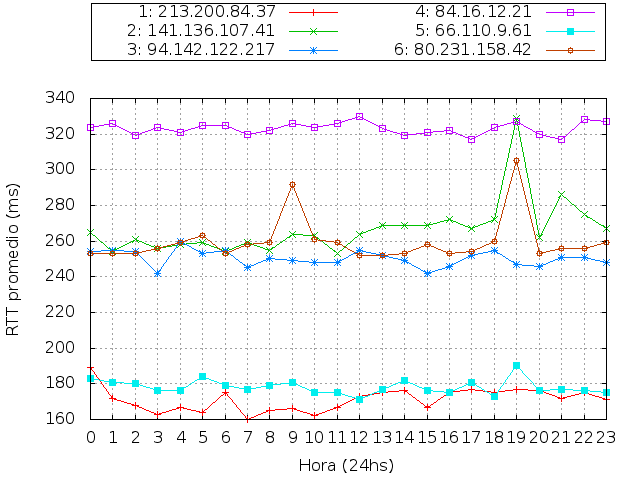
\includegraphics[width=17cm]{rtts.png}
\end{center}
\caption{Tiempo de respuesta de los enlaces transatlánticos a lo largo del día} \label{figura2}
\end{figure}

\subsection{Enlace transpacífico}

\begin{figure}[H]
\begin{center}
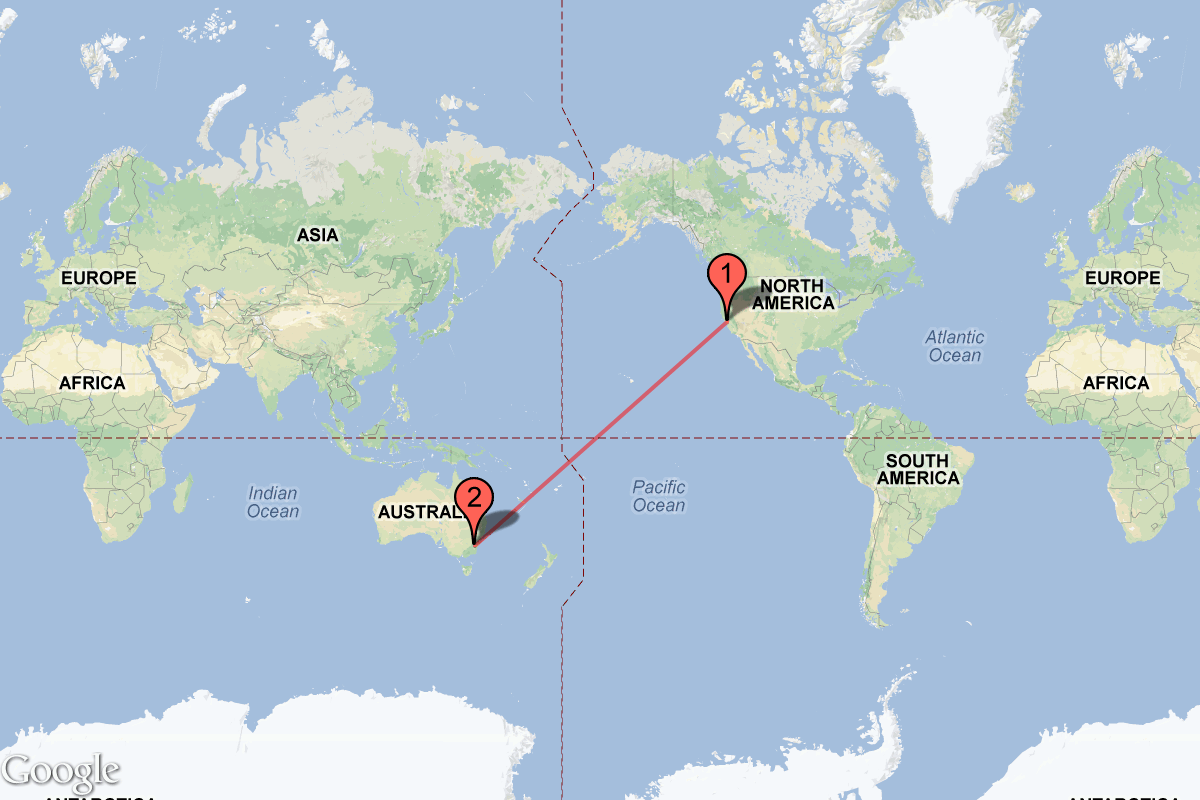
\includegraphics[width=17cm]{enlaceaustralia.png}
\end{center}
\caption{Enlace transpacífico} \label{figura3}
\end{figure}

\noindent \begin{center} \begin{tabular}{| c | c | c | c | c |} \hline 
Pin 	 & 	 Dirección IP 	 & 	 Coordenadas 	 & 	 Distancia total recorrida hasta él en Km 	 & 	 RTT mínimo en ms \\ \hline 
1 	 & 	 89.221.35.141 	 & 	 (37.9283,-122.0566) 	 & 	 11179.8250554 	 & 	 55.9 \\ \hline 
2 	 & 	 202.158.194.173 	 & 	 (-35.28,149.22) 	 & 	 24234.7289268 	 & 	 121.17 \\ \hline 
\end{tabular} \end{center}

\noindent \begin{center} \begin{tabular}{| c | c | c | c | c |} \hline 
Enlace 	 &	Distancia en Km 	& 	RTT mínimo en ms	\\ \hline 
1 - 2	 &	12222	 	 		& 	61.11				\\ \hline 
\end{tabular} \end{center}

\subsection{Variación del RTT a lo largo del día}

\begin{figure}[H]
\begin{center}
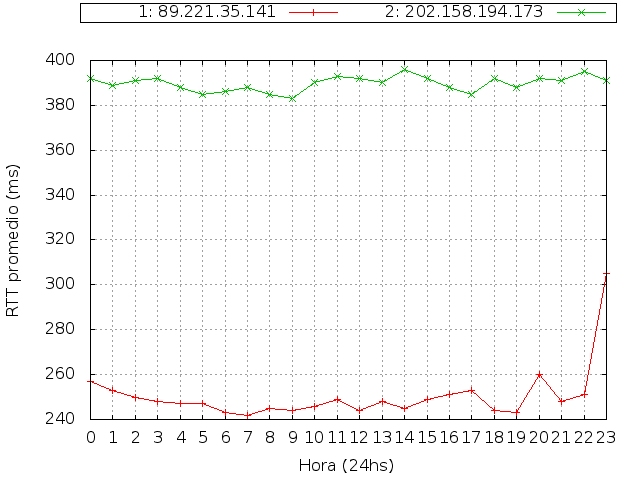
\includegraphics[width=17cm]{rttaustralia.png}
\end{center}
\caption{Tiempo de respuesta del enlace a Australia a lo largo del día} \label{figura4}
\end{figure}

\subsection{Casos curiosos}

\begin{figure}[H]
\begin{center}
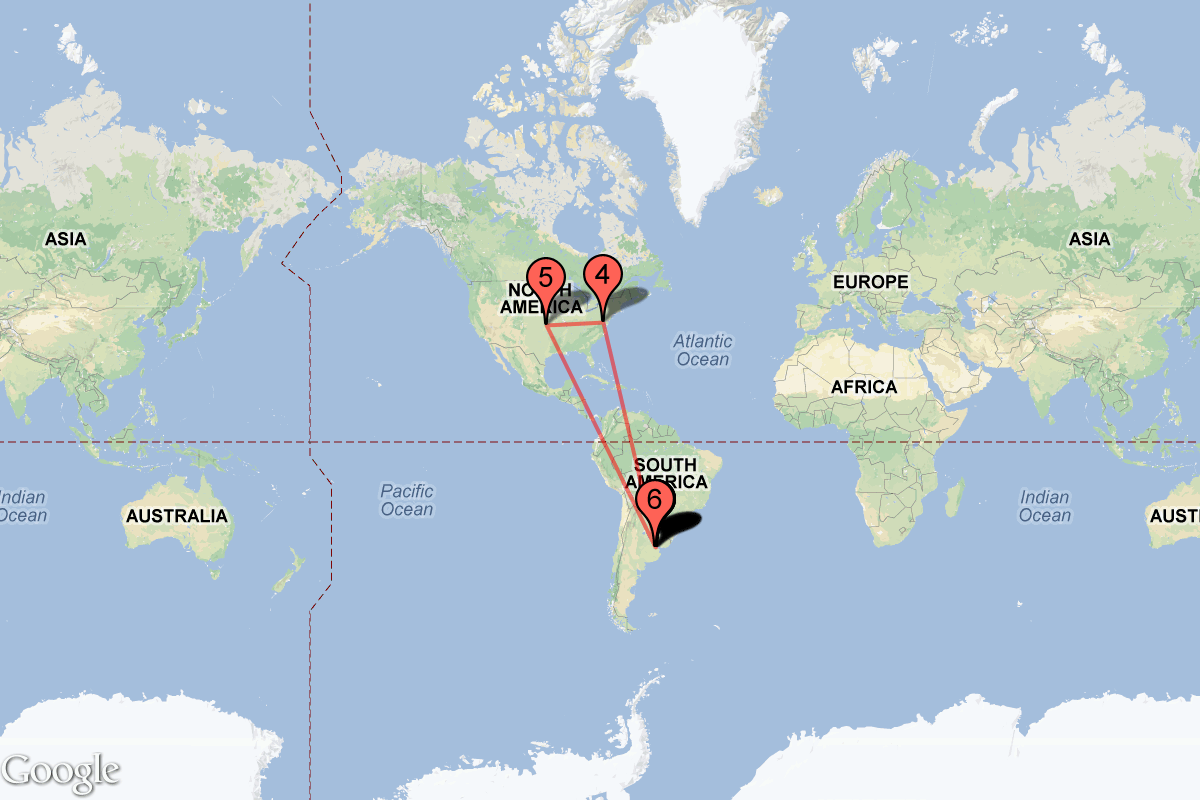
\includegraphics[width=17cm]{perfil.png}
\end{center}
\caption{Traceroute a perfil.com.ar} \label{figura5}
\end{figure}

En este caso al hacer un traceroute desde una dirección IP en Argentina a perfil.com.ar, un sitio web hosteado en Argentina, observamos que el tráfico primero se dirige a los Estados Unidos y luego vuelve al país para acceder al sitio.

\begin{figure}[H]
\begin{center}
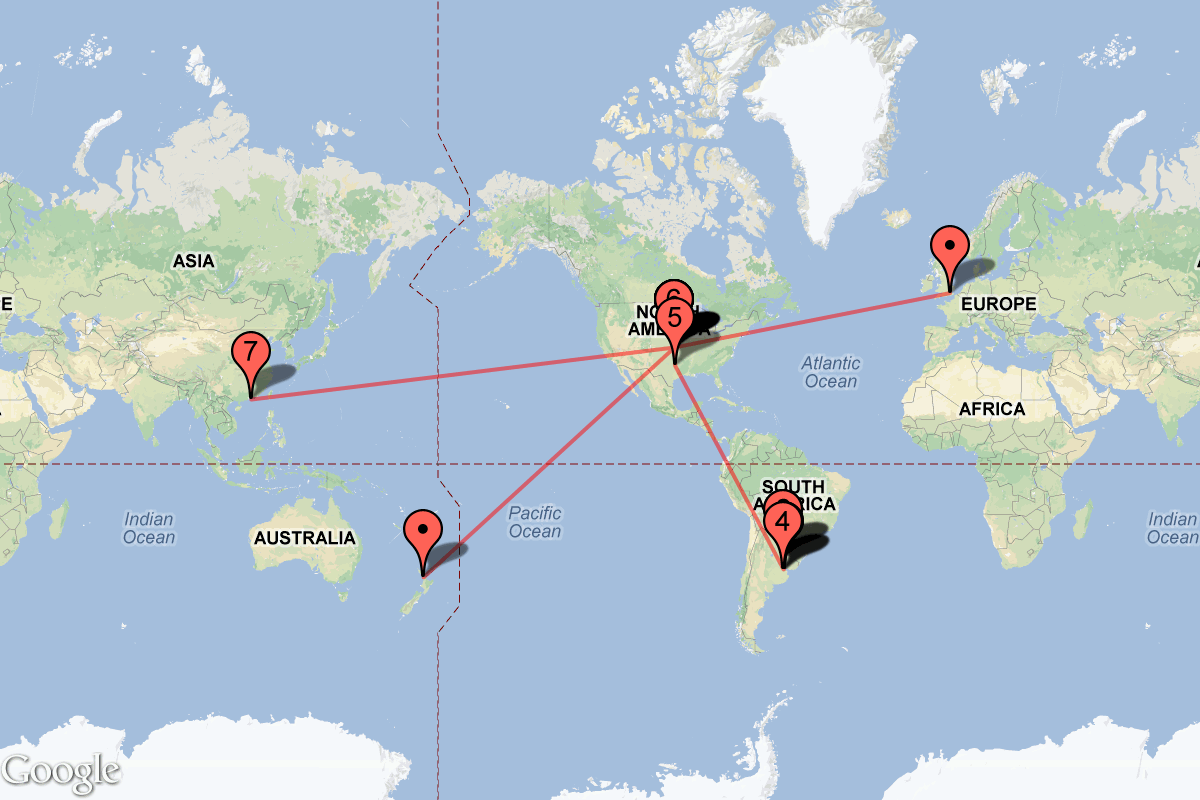
\includegraphics[width=17cm]{newzealand.png}
\end{center}
\caption{Traceroute a newzealand.govt.nz} \label{figura6}
\end{figure}

Realizamos un traceroute a una página web en Nueva Zelanda y obtuvimos que los paquetes se dirigieron primero a Estados Unidos, luego a Asia, de ahí vuelven a Norte América para dirigirse a España. Finalmente vuelven a Estados Unidos para ser enviados a Nueva Zelanda.	\\
\indent	Al intentar reproducir los resultados días más tarde no obtuvimos los mismos resultados, en una ocasión iba directo desde Estados Unidos y en otras fue a través de Asia.
